\documentclass[professionalfont]{beamer}

\usepackage{graphicx}
\usepackage{newtxtext,newtxmath}
\usetheme{default}
\usecolortheme{seagull}

\setbeamertemplate{navigation symbols}{}
\setbeamertemplate{itemize item}{\textbullet} 
\setbeamertemplate{title page}{
    \begin{center}
        {\textcolor{blue}{\textbf{\fontsize{10}{14}\selectfont MathGenie: Generating Synthetic Data with Question Back-translation for Enhancing Mathematical Reasoning of LLMs}}} \\[1.5cm]
        
        {\fontsize{9}{14}\selectfont Zimu Lu, et al \\[0.3cm]
        The Chinese University of Hong Kong \\[0.3cm]
        September 11, 2024}
    \end{center}
}
% ------------------ Title ------------------

\begin{document}
\frame{\titlepage}

\begin{frame}
\begin{center}
    { \textbf{\textcolor{blue}{ {\fontsize{12}{14}\selectfont Abstract} }} }
\end{center}
\\[0.5cm]

{\fontsize{10}{14}\selectfont 
\begin{itemize}
    \item There is a performance gap between open / closed source LLMs
    
    - New method for generating diverse and reliable math problems
\end{itemize}
\\[0.5cm]

\begin{itemize}
    \item We suggest MathGenie
    
    - This augmentation increased open-source models' performance
\end{itemize}
}

\end{frame}
% ------------------ Slide 1 ------------------

\begin{frame}
\begin{center}
    { \textbf{\textcolor{blue}{ {\fontsize{12}{14}\selectfont Introduction} }} }
\end{center}
\\[0.5cm]

{\fontsize{10}{14}\selectfont 
\begin{itemize}
    \item Three main types of solution
    
    - CoT, PoT, Code-Integrated solution
    
    - Code-Integrated solution is superior

    - MathGenie generates Code-Integrated solution
\end{itemize}
}

\end{frame}
% ------------------ Slide 2 ------------------

\begin{frame}
\begin{center}
    { \textbf{\textcolor{blue}{ {\fontsize{12}{14}\selectfont MathGenie Framework} }} }
\end{center}

{\fontsize{10}{14}\selectfont 
\begin{itemize}
    \item {\textcolor{blue}{Iterative Solution Augmentation}}: Gives variation to solutions
\end{itemize}

\begin{itemize}
    \item {\textcolor{blue}{Question Back-Translation}}: Invert solutions to questions
\end{itemize}

\begin{itemize}
    \item {\textcolor{blue}{Verification-based Solution Filtering}}: Verify question-solution pair
\end{itemize}
}

\begin{center}
    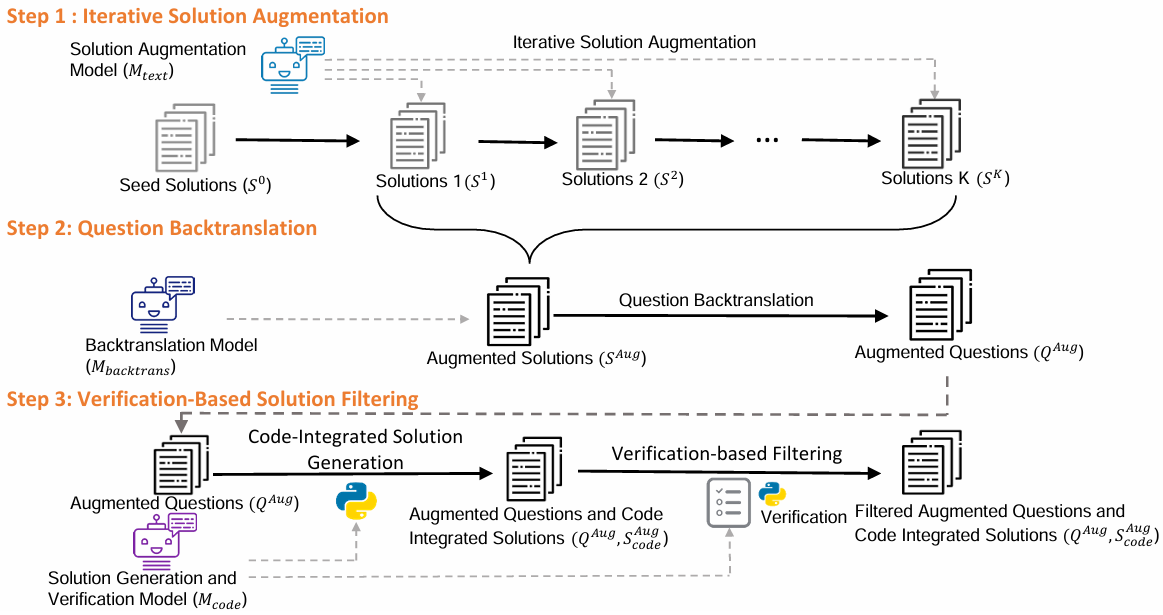
\includegraphics[width=1.0\textwidth]{figure1.png}
\end{center}

\end{frame}
% ------------------ Slide 3 ------------------

\begin{frame}
\begin{center}
    { \textbf{\textcolor{blue}{ {\fontsize{12}{14}\selectfont Question Back-Translation} }} }
\end{center}

{\fontsize{10}{14}\selectfont 
\begin{itemize}
    \item Direct Question Augmentation (Left)
    
    - It may produce question with no answer
\end{itemize}

\begin{itemize}
    \item Question Back-Translation (Right)
    
    - Correctly augments the question
\end{itemize}
}

\begin{center}
    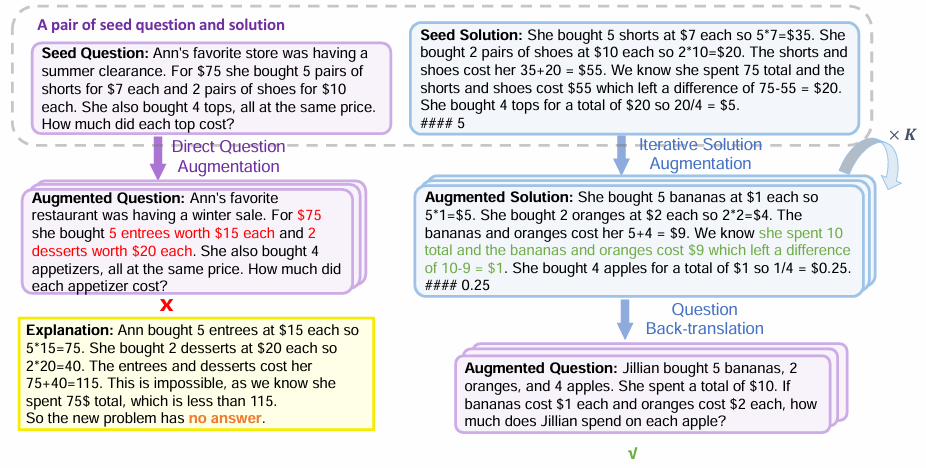
\includegraphics[width=1.0\textwidth]{figure2.png}
\end{center}

\end{frame}
% ------------------ Slide 4 ------------------

\begin{frame}
\begin{center}
    { \textbf{\textcolor{blue}{ {\fontsize{12}{14}\selectfont Experiment} }} }
\end{center}

{\fontsize{10}{14}\selectfont 
\begin{itemize}
    \item Fine-tunes pretrained models (Llama Family) with MathGenie

    - This results in {\textcolor{blue}{MathGenieLM}}
\end{itemize}

\begin{itemize}
    \item Prepare 5 datasets

    - {\textcolor{blue}{In-domain}}: GSM-8K, MATH

    - {\textcolor{blue}{Out-domain}}: SVAMP, Simuleq, Mathematics
\end{itemize}

\begin{itemize}
    \item Compare MathGenieLM with various models

    - {\textcolor{blue}{Open source}}: Mammoth, MathCoder, ToRA

    - {\textcolor{blue}{Closed source}}: GPT-3.5, GPT-4, PaLM-2
\end{itemize}
}

\end{frame}
% ------------------ Slide 5 ------------------

\begin{frame}
\begin{center}
    { \textbf{\textcolor{blue}{ {\fontsize{12}{14}\selectfont Result and Conclusion} }} }
\end{center}
\\[0.5cm]

{\fontsize{10}{14}\selectfont 
\begin{itemize}
    \item MathGenieLM achieved SOTA for open-source models
    
    - However, there was noticable gap compared to GPT-4
\end{itemize}
\\[0.5cm]

\begin{itemize}
    \item Limitation
    
    - It requires significant GPU resource
    
    - It cannot process images as input
\end{itemize}
}
\end{frame}
% ------------------ Slide 6 ------------------

\end{document}
